\chapter{Segmentação de Imagens}\label{cap:segmentacao}
A segmentação é um problema do tipo "\textit{ill-posed}" ("mal definido"), uma vez que não existe uma solução única, universal. Por isso, a segmentação é considerada o problema mais difícil de ser resolvido em análise de imagens \citep{l6}.

\section{Conceito}
A segmentação de imagens tem como uma de suas interpretações como a divisão em regiões ou categorias consideradas "relevantes", que correspondem a objetos ou partes de objetos. Decidir o que é relevante em uma imagem depende do problema a ser resolvido, em que os objetos segmentados devem corresponder às áreas de interesse da aplicação. Dentre essas aplicações, podemos citar os seguintes exemplos:

\begin{itemize}
\item Aplicações militares: Reconhecimento de alvos terrestres, aéreos e navais;
\item Análise de imagens médicas: Identificação de doenças como tumores;
\item Veículos autônomos; e
\item Robótica.
\end{itemize}

\section{Segmentação para seres humanos e para computadores}\label{sec:segmenthm}
Para seres humanos, a identificação de regiões similares ou objetos diferentes presentes em uma imagem é um processo fácil. Seu sistema cognitivo auxiliado por seu sistema visual permite reconhecer e segmentar os objetos de forma instantânea sem a percepção de todo esse processo. Além disso, o uso da segmentação por distância como técnica auxiliar é outro fator que contribui para esse processo, uma vez que sua visão estereoscópica lhes fornece informação de profundidade.
No caso de computadores, essa tarefa se torna mais complexa, pois envolve a análise de características de cada pixel ou da distribuição da população de pixels. Para isso, deve-se implementar algoritmos de segmentação, os quais serão explorados com maior profundidade nas seções subsequentes dessa pesquisa. A figura \ref{fig:Berkeley_mulher} exibe uma imagem que foi manualmente segmentada por 4 seres humanos. É possível notar que cada pessoa não identificou como "relevantes" as mesmas áreas, conforme ilustrado pela figura \ref{fig:Berkeley_mulher_segmentada}. 

% Figura 
  \begin{figure}[!htb]
       \begin{center}  
          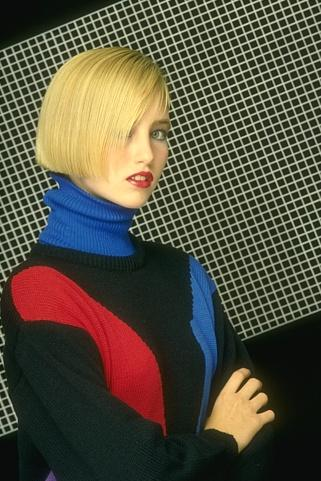
\includegraphics[width=0.3\columnwidth]{img/198023.jpg}
           \caption{\label{fig:Berkeley_mulher}Imagem original. \citep{Arbelez2011}}
           % \vspace{2.0em}
       \end{center}
   \end{figure}

 % Figura 
\begin{figure}[!htb]
 \centering
 \def\baselinestretch{1}\small\normalsize
 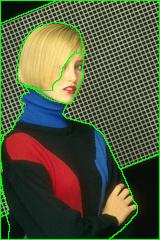
\includegraphics[width=0.2\textwidth]{img/198023-8-color.jpg}\qquad
 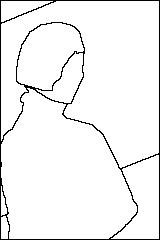
\includegraphics[width=0.2\textwidth]{img/198023-8.jpg}  \qquad
  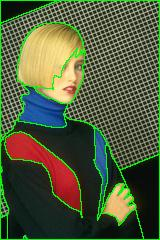
\includegraphics[width=0.2\textwidth]{img/198023-16-color.jpg}  \qquad
 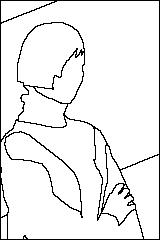
\includegraphics[width=0.2\textwidth]{img/198023-16.jpg}        
 \caption{\label{fig:Berkeley_mulher_segmentada}Imagens segmentadas por seres humanos, gerando 8 e 16 segmentos nas duas primeiras imagens e nas duas últimas, respectivamente. \citep{Arbelez2011}}
 %\vspace{2.0em}
\end{figure}


% Figura 
\begin{figure}[!h]
 \centering
 \def\baselinestretch{1}\small\normalsize
 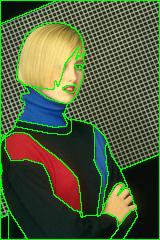
\includegraphics[width=0.2\textwidth]{img/198023-22-color.jpg}\qquad
 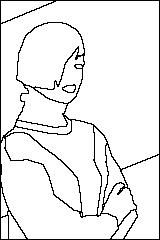
\includegraphics[width=0.2\textwidth]{img/198023-22.jpg}  \qquad
  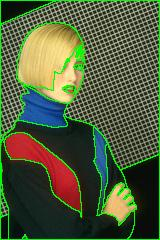
\includegraphics[width=0.2\textwidth]{img/198023-26-color.jpg}  \qquad
 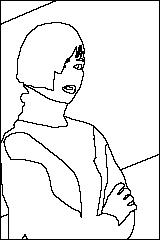
\includegraphics[width=0.2\textwidth]{img/198023-26.jpg}        
 \caption{\label{fig:Berkeley_mulher_segmentada2}Imagens segmentadas por seres humanos, gerando 22 e 26 segmentos nas duas primeiras imagens e nas duas últimas, respectivamente. \citep{Arbelez2011}}
 %\vspace{2.0em}
\end{figure}




Ainda que o processo de segmentação para humanos seja fácil e automático, é comum e natural que diferentes pessoas identifiquem objetos ou partes de objetos distintos em uma dada imagem. Isso se deve à percepção de relevância atribuída a cada região variar com a interpretação pessoal de cada um. 
O mesmo problema ocorre de forma mais acentuada com relação aos diferentes algoritmos. Cada algoritmo tem a sua própria abordagem para tratar do mesmo problema e, de acordo com sua implementação, leva a diferentes resultados, que podem ser analisados comparativamente. É importante dizer que o mesmo algoritmo pode ser mais ou menos eficiente de acordo com a imagem utilizada como dado de entrada, possibilitando diversos estudos na área como o tema desta pesquisa. A figura \ref{fig:indio} ilustra este problema\citep{berkeley} . 

% Figura 
  \begin{figure}[!htb]
       \begin{center}  
          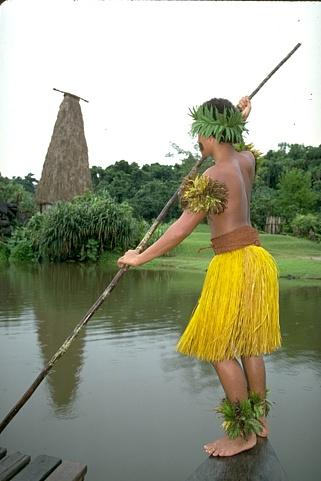
\includegraphics[width=0.3\columnwidth]{img/101087.jpg}
           \caption{\label{fig:indio}Imagem original. \citep{berkeley}}
           % \vspace{2.0em}
       \end{center}
   \end{figure}



 % Figura -----------------------------------------------------------------------------------------------------------------------------       
\begin{figure}[!htb]
 \centering
 \def\baselinestretch{1}\small\normalsize
 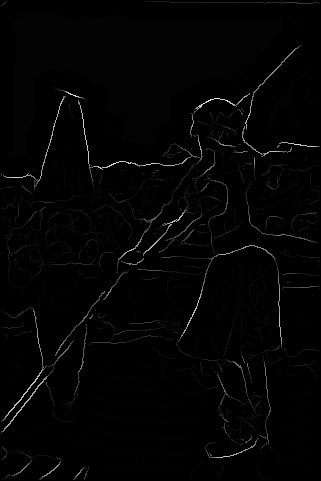
\includegraphics[width=0.2\textwidth]{img/101087-77.jpg}\qquad
 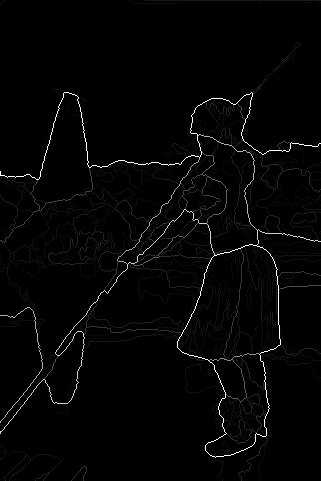
\includegraphics[width=0.2\textwidth]{img/101087-80.jpg}  \qquad 
  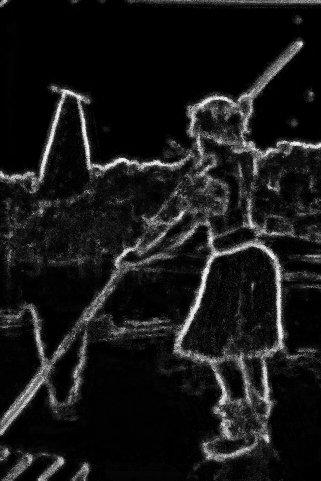
\includegraphics[width=0.2\textwidth]{img/101087-82.jpg}  \qquad
 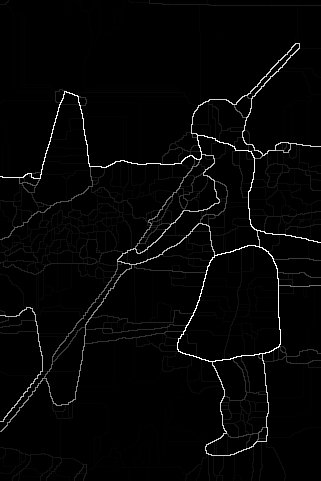
\includegraphics[width=0.2\textwidth]{img/101087-85.jpg}        
 \caption{\label{fig:indiosegmentado}Resultados de 4 algoritmo de detec\c{c}\~{a}o de bordas. \citep{berkeley}}
 %\vspace{2.0em}
\end{figure}
 % Figura -----------------------------------------------------------------------------------------------------------------------------


Devido a grande variedade de algoritmos existentes, essa pesquisa se limitará à explicação dos principais e mais utilizados, os quais fornecem um bom entendimento das técnicas utilizadas e servem como base para o desenvolvimento de novas técnicas.


